\documentclass[a4paper]{report}
\usepackage[utf8]{inputenc}
\usepackage[numbers]{natbib} % scientific references in the bibliography
\usepackage{hyperref}
\usepackage{graphicx}
%\usepackage{datetime}
\usepackage{color}
\usepackage{perpage} %the perpage package
\MakePerPage{footnote} %the perpage package command
%\usepackage{microtype}
%\usepackage{draftwatermark}
\usepackage{tikz}

\newcommand{\todo}[1]{\footnote{{\color{red} TODO: #1}}}

% ------------------------------------------------------------------------------
% Metadata
% ------------------------------------------------------------------------------
\title{Ontology Learning from Swedish Text}

\author{Jan Daniel Bothma}

% ------------------------------------------------------------------------------
% Document
% ------------------------------------------------------------------------------
\begin{document}

\maketitle

\begin{abstract}
\end{abstract}	

\tableofcontents

\chapter{Introduction}
%ONE-SENT Ontology learning learning tools significantly speed up the knowledge extraction part of the Knowledge Engineering process. I'm going to investigate ontology learning from Swedish text.
%%UU-CHAP Motivation for the Project
%%UU-CHAP Background to the problem or system
%%"I am going to look at the following things"

By encoding semantic information about the world in a form that can be processed by computers, computers can provide better support in many tasks.


\section{Semantic Web}

\section{Ontologies}

\section{Ontology Engineering}

\section{Ontology Learning}


\section{Problem}
%ONE-SENT Hoewever, there is no Ontology Learning System for learning ontologies from Swedish text.

There appears to be no ontology learning software system that has been applied to learn ontologies from Swedish text.
\todo{Hjelm's thesis\cite{Hjelm09Thesis} learnt a "prototypal" ontology from several languages including swedish.
We can learn a bit from it, but he used terms from an existing ontology, and we need to check if the relations they learnt are applicable.
Given this, this sentence might be too strong}
There are some efforts to extract semantic data from Swedish text for some specific applications and domains
\todo{maybe need to be clearer why these aren't directly suitable, domain independence etc}, but to our knowledge, these have not been combined to extract concepts and relations and induce axioms from Swedish domain text.
\todo{cite what we know about here to demonstrate we have actually done a bit of searching}

\section{Objective}

The objective of this thesis is thus to investigate the application of Ontology Learning methods to Swedish text for the construction of domain ontologies. \todo{When I've chosen the methods I'm focusing on I can probably add another line or two to be more specific and why}

\section{Research Questions}

To fulfill this objective, this report attempts to answer the following research questions:

\begin{enumerate}
  \item{What are the general requirements for ontology learning research and application?\todo{how we derived this question isn't clear from the introduction. Either this becomes a side effect part of the method, or we need to justify this "product" in the intro before the questions}}
  \item{How do common ontology learning methods need to be modified to extract ontologies from Swedish text?\todo{I think we said this was too broad and I need to replace it with a comparison between two methods when I choose them. Perhaps the idea was just to compare our work compared to some baseline?}}
  \item{How do these modified methods perform compared to \todo{some baseline??? evaluation}?}
\end{enumerate}

\section{Approach}
%ONE-SENT

This section needs to identify and show how we avoid possible sources of bias.

The basis of our method is how OL has been applied to other comparable languages like German with its compounding, and what's been learnt from the existing work on information extraction from Swedish.

The implementation should probably be based on the architecture proposed in \cite{Cimiano2009OL}

NLP tools for the common annotations are available and under further development, partly as a result of the BLARK for Swedish project.

The procedure is something like set up preprocessing, apply existing methods to swedish, evaluate, tweak for swedish, evaluate.

Ideally we can repeat an experiment for English and reproduce their results, to support the assertion that our implementation is ok.

I think I'll evaluate taxonomy extraction against the Eurovoc thesaurus since I can probably get hold of corpora for one or more of the topics they cover.

The implementation will probably be integrated with some OE system. Protege 4+ looks nice since it has decent, modern libraries and tools and plugin framework.

\section{Delimitations}

it'd be nice but I probably won't be able to ground my ontologies in any upper ontologies (ontology matching and ontological architecture). Maybe this is easy or critical and I can revise this entry.

There's a lot of research into using internet phenomena like croud sourced data and stuff. We're focusing in extracting information from any Swedish text. This means we can produce results for domains that have very little or unrepresentative data online (but depends on finding some representative corpus). These approaches also have issues like access to the services and reliability of the data. For these reasons, we're not trying the web-sourced stuff specifically.

\section{Report Structure}

\chapter{Background}
%%UU-CHAP Overview of relevant research and development that is used in specifying the problem and obtaining and evaluating appropriate solutions.
%%ONE-SENT Many methods for the subtasks have been developed for other languages, and some have already been applied to Swedish, but they have not been combined and evaluated as a pipeline. Furthermore, none of the existing OL systems are suitable to be extended to Swedish, nor support the necessary evaluation approaches.
%%UU-REQ Awareness of relevant prior research and development literature
%% -- comment on its relevance. In what way _is_ it relevant and in what way is it _not_ relevant.
%%UU-REQ critical appraisal of that literature as a basis for the formulation of project objectives and the conduct of the project.
%% -- quality of the literature affects its bearing on the project. Note on the quality of an evaluation keeping in mind whether a plain olde eval would have been suitable in the first place - what's the objective of the publication?

This chapter gives an overview of the theoretical background to this thesis.
The relationships between Ontology Learning from Text and its surrounding disciplines are identified in Sec.\ref{sec:lit-rev:parents}, then work and issues relevant to this field and this thesis specifically are discussed in Sec.\ref{sec:lit-rev:immediate}.

\section{Parent disciplines}
\label{sec:lit-rev:parents}

This section identifies the relationships between Ontology Learning from Text, and the surrounding disciplines.
At a high level, Knowledge Management and the Semantic Web form the basis of applications that are supported by semantics encoded in a manner that allows automated reasoning.
Ontology Learning is related with Knowledge Acquisition and Representation as a specific form of these processes, and the relation between Machine Reading and Ontology Learning is covered briefly.
Some of the parts Ontology Learning plays in Ontology Engineering are identified, and finally the broader field of Ontology Learning is described, leading to a definition of Ontology Learning from Text.

\begin{figure}
  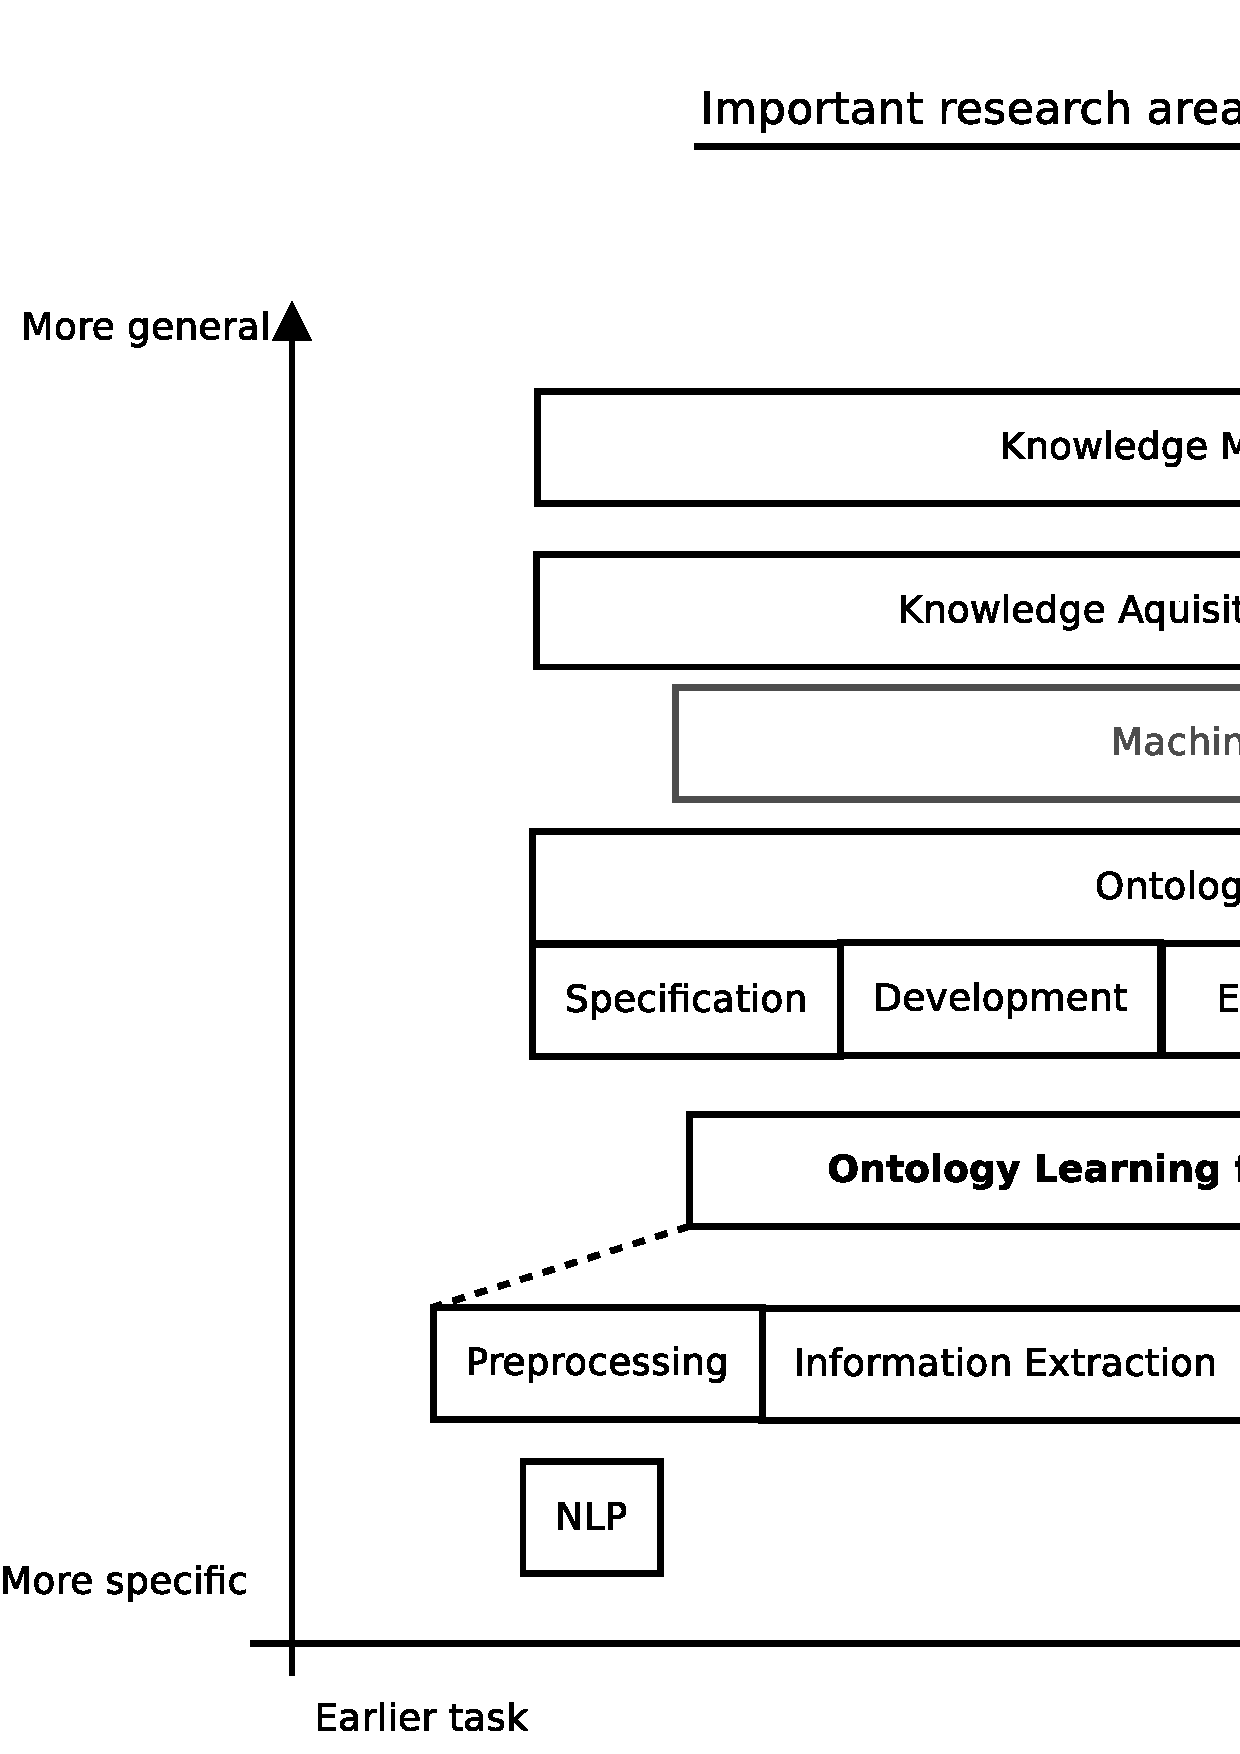
\includegraphics[width=\textwidth]{graphics/related-research-fields.png}
  \caption{Related research fields}
  \label{fig:related-research}
\end{figure}



\subsection{Knowledge Management}

Knowledge Management involves creation, storage, retrieval, transfer and application of the tacit and explicit knowledge pertaining to an organisation \citep{AlaviLeidner2001KM}.
Knowledge has been shown to be a significant asset in organisations, and information technology can help making such knowledge available to areas where the knowledge is not transferred easily \citep{AlaviLeidner2001KM}.

An example of using information technology to collect, store and apply valuable organisational knowledge is the \emph{semantically enabled} IURISERVICE iFAQ database of legal questions and answers given by experienced Spanish judges.
This tool aims to support inexperienced judges in answering legal questions\cite{IURISERVICEPerformance2007}.
Important terms in the questions and answers are associated with their synonyms and the domain of law that they apply to.
When a question is entered to search for related question-answer pairs, the semantic information is used to improve the results over a plain text search, even when considering different forms of the words in the query.
The query is expanded to include exact matches, morphological variations\footnote{In the linguistic sense, such as \emph{car} to \emph{cars} for plurality}, and synonyms.
The similarity of the result questions to the query question is then calculated, considering the similarity of concepts and the grammatical structure of the questions, to provide the most-similar results to the user.
The semantic information is further used to provide suggestions of relevant legal cases whose decisions might have an impact on the issue at hand.

\subsection{Semantic Web}

By making semantically annotated information available over the internet, many resources can be combined to support complex tasks involving many parties.
The Semantic Web\footnote{http://www.w3.org/2001/sw/} is the manifestation of this.
In a hypothetical example, Tim Berners-Lee et al. \footnote{Tim Berners-Lee, James Hendler and Ora Lassila. The Semantic Web. \emph{Scientific American}, 284(August), 2001} describe a scenario where a brother and a sister try to book medical appointments for their mother with a nearby treatment centre available to their mother's health insurance policy, on dates that they can alternate driving their mother.
Information about their availability, the clinics (including treatments they offer and their schedules) and the insurance policy must be available to the computers involved in proposing a solution.
Furthermore, the meaning of this information, and how it relates to the other information involved in the computation, must be available.
For example, the computer must be able to distinguish between the treatment centre's postal address and their visiting address.
This information is encoded in ontologies and mappings between semantic entities in standardised formats such as OWL\cite{OWLOverview2004} to support this interoperability.

The masses of information available as plain text is not directly usable in the semantic web.
Knowledge must be encoded in machine-readable forms compatible with the Semantic Web.
That knowledge can come from a variety of sources, and the process of gathering knowledge for storage and application in semantically-enabled systems is known as Knowledge Acquisition.

\subsection{Knowledge Acquisition}

Knowledge Acquisition in the context of information technology is the elicitation and interpretation of knowledge about a particular domain for use in knowledge-based systems \citep{anjewierden1987KATools}.
This corresponds to the acquisition part of Knowledge Management and is a precursor to Knowledge Representation. 

\subsection{Knowledge Representation}


\subsection{Ontologies}
\label{sec:lit-rev:ontologies}

A commonly-cited definition of ontologies in the field of knowledge engineering is as \emph{``a formal, explicit specification of a shared conceptualization''} \cite{StuderEtAl1998KEPM}.
Here, a \emph{conceptualization} is the objects, concepts and relations between them, in an abstract view of the world intended for a particular purpose.
The conceptualization should be \emph{shared} within the context of its application.
The objective with this explicit specification is to allow computer agents to operate on this view of the world or for its integration in human-operated software.

Ontologies that represent a particular domain are known as \emph{Domain Ontologies}.
One way to support integration of several domain ontologies is by defining elements common to many domains in an \emph{upper ontology}\cite{SemanticIntegration2004Noy}.

\todo{could distinguish between "lexical" and non-lexical ontologies like what Hjelm and I think Cimiano refers to.}

\subsection{Ontology Engineering}

The discipline of specifying, developing, introducing and maintaining ontologies for some application is known as \emph{Ontology Engineering} (OE)\cite{HOO2009OntEngMeth}.
Along with broader considerations of OE such as the intended users and software engineering issues, the domain expert(s) and ontology engineer must gather relevant domain knowledge (Knowledge Acquisition) and encode it in a computer-readable form (Knowledge Representation)\cite{OntMethOverv1999}.
This is challenging and repetitive and is known as the Knowledge Acquisition Bottleneck\cite{OLforSemWeb2001}.
As an example, a "tasks and skills" ontology in the case study in \cite{HOO2009OntEngMeth} consisted of about 700 concepts after refinement. 
Automating as much as possible of the knowledge acquisition and representation can reduce the effort for domain experts and ontology engineers when developing and maintaining ontologies\todo{need to back this up}.

\subsection{Ontology Learning}

The automatic or semi-automatic construction of ontologies from domain data is called Ontology Learning \cite{Cimiano06}. 
Ontology Learning (OL) can start with structured, semi-structured or unstructured data as input \cite{Cimiano2009OL}.
Structured data, such as databases, can be somewhat independent of language and its semantics are described by its schema or structure \todo{I think \cite{Cimiano2009OL} is sufficient but need to check}.
Most methods for ontology learning from semi-structured data such as wikis and unstructured data in the form of plain text depend on preprocessing techniques from the field of Natural Language Processing (NLP) to provide syntactic annotations like part of speech or syntactic dependencies.
OL methods are then applied to the annotated corpus, each method extracting one or more kind of ontology element.

Ontology learning software systems have been implemented that provide one or more algorithms for extracting concepts, relations and axioms from a text corpus.
Such systems are often integrated with dedicated NLP tools to provide the required preprocessing facilities.
Extracted elements are manually or automatically added to an ontology and can often be output in a standard ontology serialisation format like OWL\cite{OWLOverview2004}.

Ontology learning methods have varying degrees of language dependence. 
In the simplest case, an OL system can be applied to another natural language by replacing the language models in the NLP components with models trained on the other language. 
However, often the syntactic and semantic structure of languages vary enough to require modifications to OL methods or the process as a whole \cite{Voelkner2008Spanish}\todo{saying "often" probably means we need more than one example}.

\subsection{Ontology Learning from Text}

This section defines Ontology Learning from text and discusses important work in this field. More detail of the tasks and methods of Ontology Learning from Text is covered in Sec.\ref{sec:lit-rev:immediate}

Ontology Learning from Text is the process of building a formal ontology from a semi-structured or unstructured text corpus from a particular domain \citep[p.3-7]{Cimiano06}.
The ontology is intended to model the concepts and the semantic relationships between the concepts in the domain.
Ontologies are further described in Sec.\ref{sec:lit-rev:ontologies}. 

The typical tasks and their outputs are shown in Fig.\ref{fig:output-task-technique}. 

\begin{figure}
  \includegraphics[width=\textwidth]{graphics/output-task-technique-WongLiuBennamoun.png}
  \caption{Tasks, techniques and outputs in ontology learning. \cite{Wong2009PhD}}
  \label{fig:output-task-technique}
\end{figure}


\subsection{Machine Reading}

Machine Reading is the automatic, unsupervised \emph{'understanding'} of text where understanding means formation of beliefs supporting some level of reasoning from a textual corpus \citep{EtzioniEtAll06MachineReading}.
Machine Reading is distinguished from Information Retrieval where this is done in a in a highly supervised, manual manner - for example where patterns for extracting desired entities are hand-written or manually selected from an extracted list.
Machine reading strives instead for extracting arbitrary semantic relations without human supervision \citep{EtzioniEtAll06MachineReading}.

While Cimiano concluded that some level of supervision is necessary in Ontology Learning from Text \citep{Cimiano06}, recent work in Ontology Learning from Text such as OntoUSP\citep{Poon2010OntoUSP} and OntoCMaps \citep{Zouaq11OntoCmaps} shows progress towards learning arbitrary relations with high precision and recall in an unsupervised manner, which is much closer to machine reading than earlier work in the field.


\section{Immediate discipline}
\label{sec:lit-rev:immediate}

This section describes relevant research in ontology learning from text.
The descriptions are organised according to the role the research plays within the field and its processes.

The key issues for ontology learning from text are shown in \ref{fig:ol-issues}.
OL from text starts with collecting and preparing text corpora. The corpora must be preprocessed as needed by the information extraction methods. Evidence for potential ontology elements might be combined from various methods with overlapping scope. An ontology is constructed using the extracted information, which is generally evaluated during or following construction. As with ontology engineering, change management and user interaction are important aspects throughout the process.

Methods were chosen for inclusion in this review based on their relevance to this thesis and research in general.
While ontology learning from text includes extraction from structured text, this thesis avoids the specificity of methods for structured data.
Domain independent methods are preferred over domain-specific such as \cite{LeeEtAl03OLMed} for medicine.
Methods depending heavily on existing knowledge bases are avoided such as \cite{Gulla08LOUIE} for its dependence on film knowledge bases or \cite{Drumond10PREHE} and \cite{HaiTaoEtAl08Clonto} for dependence on WordNet\cite{Fellbaum98WordNet}.
While general domain knowledge bases such as WordNet and Cyc\cite{Lenat95Cyc} can help extract so-called \emph{low hanging fruit} and there even exists a WordNet for Swedish\cite{Viberg02SWordNet}, it generally takes a lot of effort to extend such databases to a new domain \footnote{This is in fact closely related to OL for domain ontologies} and they might introduce errors since the senses of words and phrases in specific domains might be different from those in general language.
Their consideration is left for further research.

\begin{figure}
  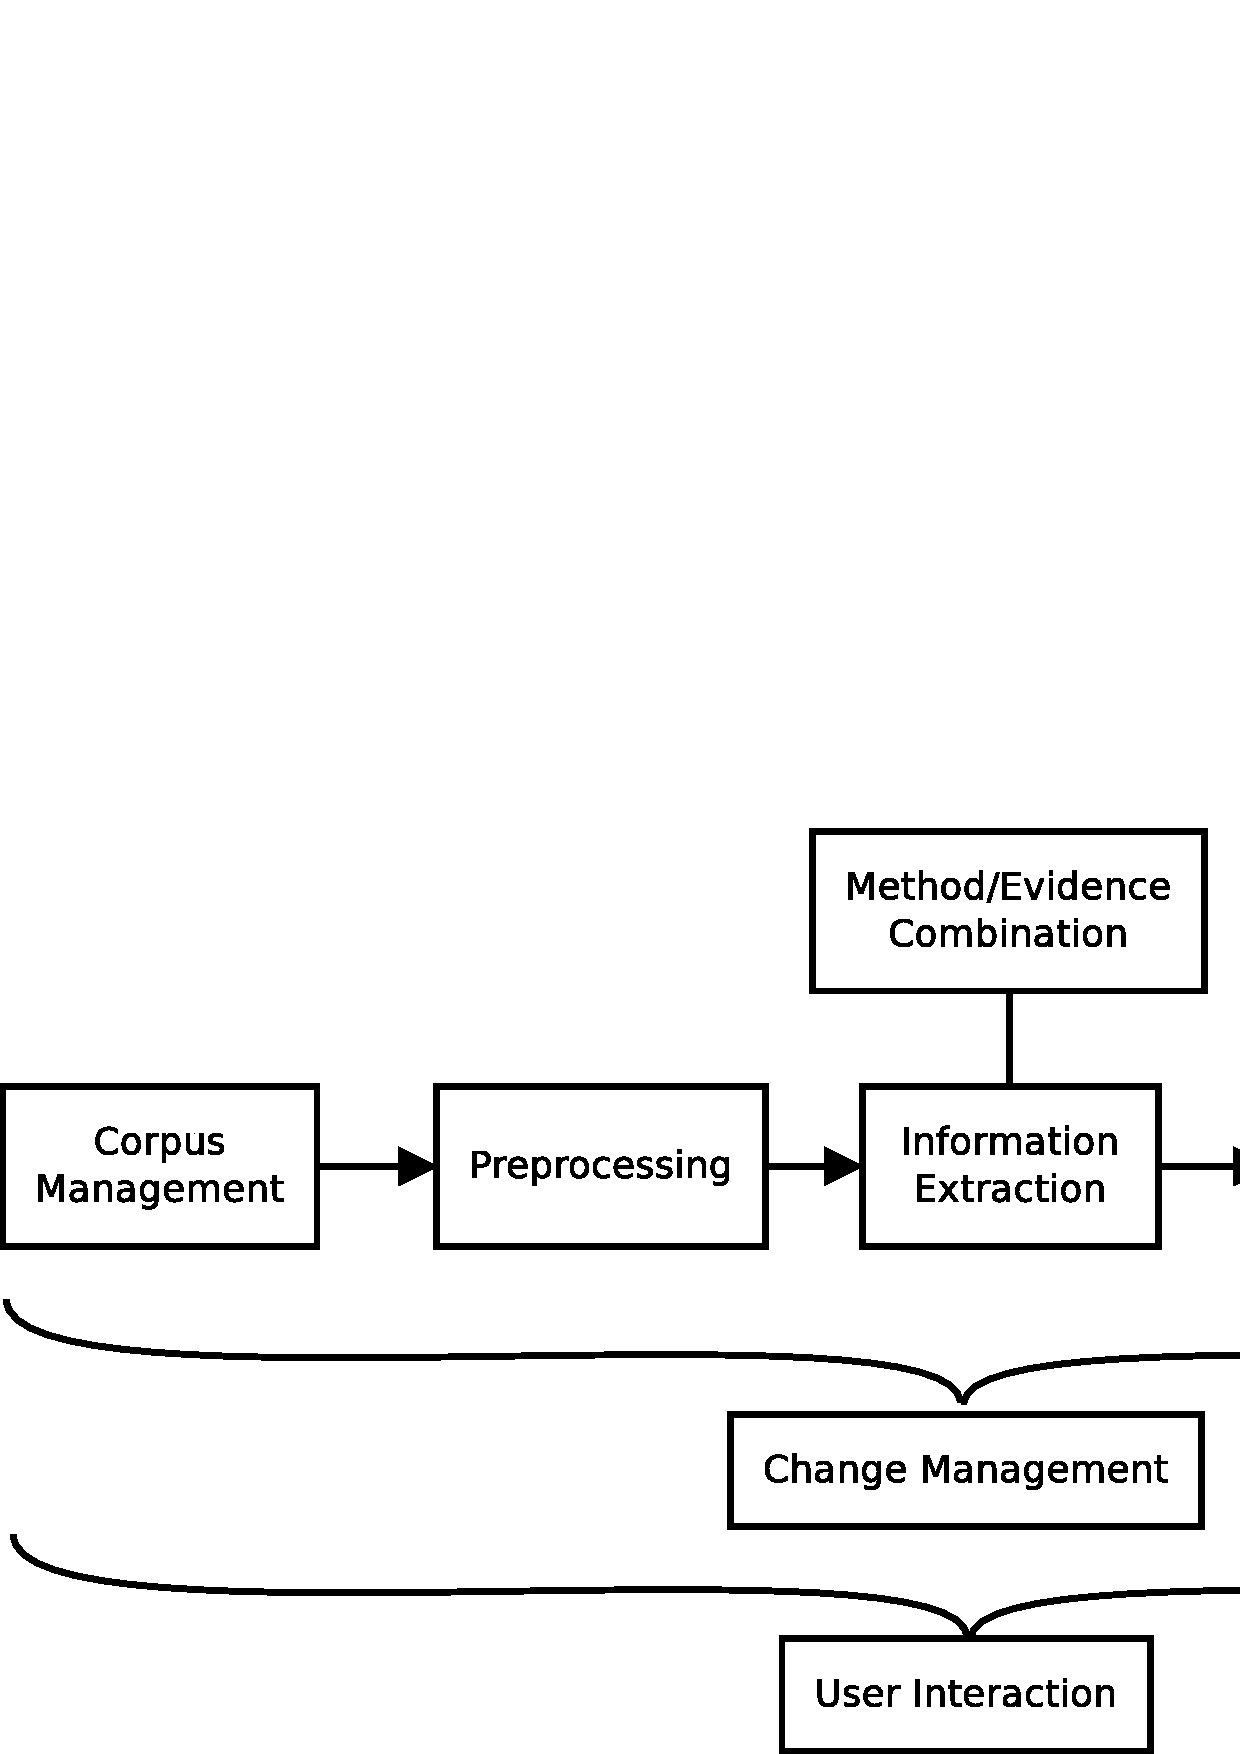
\includegraphics[width=\textwidth]{graphics/ontology-learning-system-issues.png}
  \caption{Issues for Ontology Learning systems}
  \label{fig:ol-issues}
\end{figure}

\subsection{Ontology Learning Steps}

\subsection{Corpus Management}

Corpus management involves selection of suitable corpora and storage of changes and annotations made during Preprocessing and Information Extraction.
A corpus is a collection of documents compiled for linguistic investigation or processing \citep{KokkinakisGerdin10MedCorp}.
When performing ontology learning from text, a corpus must be compiled which contains the text from which the domain model must be extracted.
Selection of suitable corpora is important since the authority of the derived ontology depends on the authority and relevance of the source text for the domain.
Annotations are generally made by NLP tools to identify linguistic features of text such as parts of speech or syntactic dependencies.
These features are then used by one or more information extraction techniques.

Maintaining the annotations of these features in the context they occur in, as opposed to simply extracting fragments and their features to a database, is necessary for some information extraction methods\citep{Frantzi98CNCValue, NenadicEtAl02TermSim, Srikant95GenAssocRul} and helps with ontology learning evaluation and research.

Many annotation formats exist including XML, other plain text formats and more complex binary formats.
Various NLP tools such as the Stanford parser \citep{Marneffe06StanfPars} and FM-SBLEX morphology tools support input and output in XML and several other formats for different applications. 
A common plain text annotation format consists of one token string and its corresponding annotation on the same line, with only one token per line.
This format is output by the HunPos tagger, for example, and can be accepted as input by MaltParser\citep{Nivre06maltparser} and FM-SBLEX. 
XML facilitates programmatic transformation and processing, although the XML schemas vary significantly meaning tools are often not directly compatible.
For example, the XML formats of the Genia corpus \citep{KimEtAl03GeniaCorpus}, the FM-SBLEX tools and the Stanford NLP tools are significantly different.\todo{Add CoNLL format\citep{NivreEtAl07NoNLL} used by \citep{Nivre06maltparser}}.

Existing corpora and common document formats often already contain features and annotations that can be useful in ontology learning.
For example, section headings can be extracted from HTML, PDF and Word documents, and coreferences (See Sec.\ref{sec:lit-rev:preproc}) are identified using XML in the Genia corpus.
GATE can accept a variety of input document formats and normalises the structure of non-plain-text formats like HTML, Microsoft Word documents and PDF to its internal annotation format with common labels for annotation types among all normalised input formats \citep{Cunningham2011GATEBook}.
The Korp annotation pipeline can accept various XML formats, and strip, copy or ignore and in some cases use existing annotations \cite{Borin12Korp}.

The multitude of annotation formats forming input and output of the numerous tools creates a challenge for corpus management.
GATE helps deal with this challenge with over ten years of refinement. 
The GATE Developer application provides user interfaces to review and edit annotations manually, while the GATE Embedded Java libraries can be used programmatically to integrate various NLP tools during preprocessing and annotation.
References to annotations can be stored by external applications to retrieve annotations for the change management tasks.

\subsection{Preprocessing}
\label{sec:lit-rev:preproc}

Preprocessing is the task of ensuring the corpus is in a suitable state for the information extraction methods to be effective, and annotating the corpus with linguistic features needed by certain information extraction methods.
Common preprocessing tasks for ontology learning include
\begin{itemize}
  \item tokenisation
  \item sentence splitting
  \item part of speech and morphology analysis
  \item lemmatisation or stemming
  \item named entity recognition
  \item coreference resolution
  \item chunking
  \item syntactic dependency parsing
\end{itemize}
An additional task of \emph{compound splitting} is important for languages where compound words are common without a separating space or hyphen, such as Swedish, German or Russian.

\subsubsection{Tokenisation}

Tokenisation identifies individual word units - mainly separated by spaces but possibly also punctuation characters.
Many NLP methods operate on individual tokens in the corpus.
For example, a part of speech tagger assigns a part of speech to individual tokens, perhaps taking the sentence context into account.
In certain domains word units might include characters that would be classed as token separators in common natural language.
Generic tokenisation methods might need modification when performing ontology learning on such domains.

\subsubsection{Sentence splitting}

Sentence splitting identifies individual sentences - sometimes taking document layout into account to improve accuracy when full-stops are missing, in headings, for example.

\subsubsection{Part of speech and morphology analysis}

Part of speech tagging, or POS-tagging, assigns grammatical word categories to individual words or other tokens such as numbers.
A tagset defines how certain features are represented.
For example in the Penn Treebank tagset, a singular common noun is tagged NN, while a plural common noun is tagged NNS \citep{Marcus93Penn}.
Tagsets often include morphosyntactic categories such as gender, number and case.

Two interchangeable tagsets are commonly used for swedish: the PAROLE tagset and the SUC tagset \citep{Forsbom08Tagging}.
A mapping is available between these tagsets \footnote{http://spraakbanken.gu.se/parole/tags.phtml}.
These tagsets support common morphosyntactic categories, for example a common singular indefinite noun of neuter gender in the nominative case such as \emph{raketvapen} (english \emph{missile}) would have the tag {\tt NCNPN@IS} in the PAROLE tagset and {\tt NN NEU PLU IND NOM} in the SUC tagset.

Many taggers are available, and they can often be configured to use custom language models. Such language models are specific to the language being tagged and are usually generated from a treebank - a corpus with annotations produced with high-enough accuracy to be used as training data for building language models and performing linguistics research.
Models for tagging Swedish text are available from Eva Forsbom \footnote{http://stp.lingfil.uu.se/~evafo/resources/taggermodels/models.html} and Beata Megyesi \footnote{http://stp.lingfil.uu.se/~bea/resources/} and embedded in the Korp pipeline. \todo{maybe something about tagger accuracy, some literature, this is lit-rev after all}

\subsubsection{Lemmatisation and stemming}

Lemmatisation and stemming both attempt to normalise words from their inflected forms to some common form.
Stemming removes common prefixes and suffixes, leaving the 'stem' behind which may not be a word in the language, for example changing \emph{kloster} and \emph{klostret} (\emph{monastery} and \emph{the monastery} respectively) to \emph{klost}.
Lemmatisation modifies words to their lemma, or uninflected form, changing \emph{klostret} to \emph{kloster} and leaving \emph{kloster} as it is.

Lemmatisation is preferred in ontology learning since it is useful to distinguish different senses of a word while coalescing different inflections of the same sense.
Stemming is usually quite a course, rule-based approach which can lose important parts of words that look like pre- or suffixes but are part of the lemma \todo{ought to cite this, \citep{Gacitua08OntoLancs} says \citep{Alkula01MeaningWords} deals with this.}, meaning many more senses of the same word would be coalesced than with lemmatisation.
The Saldo lexicon \cite{Borin09Saldo} goes a step further, by assigning unique identifiers based on the lemma to distinguish between different senses of words with the same lemma.

When lemmatising words, the appropriate sense of the word must be chosen to select the correct lemma.
Unsupervised preprocessing means that a native speaker is not available to identify the sense of the word by its meaning.
The Korp pipeline attempts to improve sense selection by choosing the sense with the most-similar morphology, such that a noun would be chosen over a verb given a word tagged as a noun, for example.

The FM-SBLEX word analysis tools and the Korp pipeline are based on the Saldo lexicon.
The FM-SBLEX tool can lemmatise words not in the lexicon, such as \emph{kommunerna} (english \emph{the municipalities}).


\subsubsection{Named Entity Recognition}

\subsubsection{Coreference Resolution}

\subsubsection{Chunking}

Chunking, or shallow parsing, identifies non-overlapping parts of sentences playing various roles in the sentence, for example identifying the noun phrases making the subject and object parts in the sentence.
The SweSPARK chunker employs a parser for chunking Swedish text \cite{Megyesi02Thesis}.

\subsubsection{Syntactic Dependency Parsing}

The OntoUSP \citep{Poon2010OntoUSP} method and the methods in the OntoCMaps system \citep{Zouaq11OntoCmaps} make use of syntactic dependencies for identifying roles of phrases in the corpus.

\subsubsection{Compound Splitting}

FM-SBLEX provides compound analysis, giving sets of two or more word senses from its lexicon that might have been compounded to form the word in question.

The relation extraction method in \cite{Kokkinakis08SolidComp} used a glossary of domain terms to select likely compound parts from the possible part pairs.

A statistical model of the swedish language is used in \citep{Sjobergh04Compounds} to split compounds. This was used for the Swedish compund splitting in \citep{Hjelm09Thesis}.

\subsubsection{The SVENSK language processing toolbox for Swedish}

SVENSK is a language processing toolbox for Swedish developed in the late 1990s and 2000\cite{OlssonGamback00SVENSK}. SVENSK aimed to support research and teaching which depended on Swedish language processing by providing common text processing tools such as taggers and parsers in a general purpose language processing framework. SVENSK was based on the GATE language processing framework.

\subsection{Information Extraction}

\todo{should probably include TextRunner/ReVerb since \cite{Poon2010OntoUSP} says its the state of the art in IE. At least the ReVerb website only mentions English}

\subsubsection{Method / Evidence Combination}

\subsection{Ontology Construction}

\subsection{Ontology Evaluation}

\subsection{Change Management}

\subsection{User Interaction}

\subsection{Ontology learning systems}

\subsubsection{OntoUSP}

OntoUSP is an ontology learning system and method which builds a \emph{probabilistic ontology} from dependency-parsed text\cite{Poon2010OntoUSP}.
It builds an ontology comprising of concepts, relations, IS-A (subconcept) and IS-PART relations between relations.
OntoUSP builds on the USP (Unsupervised Semantic Parsing) system\cite{Poon09USP}.
Both these systems use Markov Logic networks to determine the most probable parse of the corpus as a whole\todo{explain this more}.
OntoUSP achieved significantly higher precision and recall than the state of the art in the field of information extraction and question answering systems in an evaluation using the GENIA\citep{KimEtAl03GeniaCorpus} corpus\cite{Poon2010OntoUSP}.
I discovered by email correspondence with Hoifung Poon, PhD (2012-02-29) that the Stanford parser\cite{Klein03PCFGParser} used for annotating the corpus in this evaluation was trained on the GENIA Treebank\cite{Tatseisi05GENIATB}.
For this reason, it is unclear how well OntoUSP would perform using a general domain parser, or whether the other systems in the evaluation were also trained for this domain.
This is important since domain-specific parsers or treebanks are not normally available, and this treebank was constructed from the GENIA corpus.

\section{Open research areas}

The literature identifies many open research areas in OL. These have been organised into the following areas and are discussed further below:

\begin{itemize}
\item New and improved methods
\item Change management
\item Corpus quality
\item Evaluation
\item Cross-language OL and currently-unsupported languages
\item Exploit structured and web data
\item Bootstrapping models and parameter optimisation
\item Target application
\end{itemize}

\subsubsection{New and improved methods}

New methods and improvements in existing methods mean that research in this field is ongoing and requires tool support.
Methods research is commonly accompanied by experimental evaluation to show superiority in some desirable aspect\cite{Basili96Experi}.
For example, OntoUSP and OntoCMaps recently showed significant improvements over the state of the art using novel methods of identifying important relations.


\subsubsection{Change management}

Change management for ontology evolution can involve organisational practices and ontology learning tools. The environment around the ontology is often not stable \cite{Blomqvist09Thesis}. Once deployed in an application, changes might need to be applied in a controlled manner to evaluate and understand the effects of keeping the ontology up to date with its environment\cite{HOO2009OntEngMeth}. Depending on the agility of the organisation, manual evolution of the ontology might not be sufficient\cite{Blomqvist09Thesis}. \cite{Cimiano2009OL} states "As the underlying data changes, the learned ontology should change as well and this requires not only incremental ontology learning algorithms, but also some support for ontology evolution at the ontology management level".

\subsubsection{Corpus quality}

Corpus quality is a concern with regard to the validity of the learned ontology, as well as to the suitability of a given corpus for chosen OL methods. Many methods rely on large corpora \cite{Cimiano06} and the internet makes a huge variety of sources of information available \cite{Wong11Survey}. However, one might question the authority of information gathered from the internet, especially from the increasing trend of using socially generated data \cite{Wong11Survey}. It was shown in \cite{Hjelm09Thesis} that useful results could be obtained from a corpus of Wikipedia articles. They further expect that a bigger corpus would improve the recall of their classifiers and lexico-syntactic patterns but are concerned about the ambiguity introduced by a more general corpus. 

\subsubsection{Evaluation}



\subsubsection{Cross-language OL and currently-unsupported languages}



\subsubsection{Exploit structured and web data}



\subsubsection{Bootstrapping models and parameter optimisation}



\subsubsection{Target application}



\chapter{Methods}

This chapter introduces relevant research method theory and the methods applied in this thesis.

\section{Research methods}

Conflicting philosophical perspectives on research exist.
The positivist perspective asserts that knowledge of the reality which exists apart from the researcher is gained through observations.
This perspective tends to favour quantitative methods of data collection and analysis.
Positivist approaches begin with a theory which is then supported or contradicted by the evidence.
\cite[p.6-7]{creswell2003research}\todo{perhaps update to Creswell 2009}
The interpretivist perspective builds a theory out of the understandings and views of individuals.
This perspective tends to use qualitative methods, engaging with human subjects to gain knowledge.
\cite[p.7-9]{creswell2003research}
\footnote{One might note here that these philosophical views of knowledge about the world are also issues for ontology in the philosophical sense and thus for ontologies modelling reality \cite[p.6]{creswell2003research}\cite{sep-hermeneutics}.
This thesis uses the "shared conceptualisation" definition of ontologies derived from natural language.
While ontology learning from text is not a scientific research methodology in itself, in this form it bears strong similarity to interpretivist methods of knowledge acquisition}
\todo{I should probably talk about mixed methods too, since it very much exists and is probably more what I'm doing}

In Computer Science, as in other fields, the suitability  of the method depends on the questions being answered or problems tackled by the research.
When theories are difficult or impossible to prove logically, they can still be explored and supported by scientific experimentation \cite{Blomqvist09Thesis,Crnkovic2002SciMethCS}.
\todo{possibly expand on this. right now it seems like it's just dumped here out of context. expanding on experimental impl and eval in OL might help}

The outputs of research in the field of Ontology Learning from text are generally new or improved ontology learning methods, algorithms, software systems or approaches for the evaluation of the above \cite{Wong11Survey}.
Similarly to evaluation in ontology engineering, ontology learning is generally evaluated with respect to a specific application, the coverage of the modeled domain, or according to a predefined set of criteria \cite{Wong11Survey}.
\todo{perhaps expand on these. bring out the issue of mutliple corpora and gold standards and (un)generalizability (but evidence towards it)}
While quantitive methods are valued for the ease with which OL methods can be compared according in various aspects, the fact that human experts are generally needed to verify the accuracy of the model means there is an intrinsic qualitative part to ontology learning evaluation \todo{cite this synthesis/opinion/whatever}.

The objectives of this thesis are to investigate Ontology Learning from Swedish texts and identify areas of further research.
This thesis focuses on identifying existing usable tools and methods and the implementation of prototype OL system for Swedish text.
The implementation should be evaluated in its ability to produce domain ontologies in accordance with evaluation techniques for similar systems for other languages.
This thesis should also identify issues for further research in OL from Swedish text.
These issues shall be grounded in the literature, the limitations identified in the prototype system, and in the experience gained during implementation. \todo{this is still rather rough, isn't it?}

This thesis takes a \emph{system development} approach to studying the problem at hand.
This approach is relevant since the objective of this thesis is also to learn more about a problem area by planning, constructing and evaluating a prototype information system \cite{NunamakerChen90SDResearch}.
A related approach from the action research perspective\cite{BursteinGregor99SDResearch} was taken to evaluate a significant piece of research in OL which was closer to the organisational context\cite{Blomqvist09Thesis}.

Five criteria of conformance are provided for system research in \cite{NunamakerChen90SDResearch}:
\begin{enumerate}
\item The purpose is to study an important phenomenon in areas of information systems through
system building
\item The results make a significant contribution to the domain
\item The system is testable against all the stated objectives and requirements
\item The new system can provide better solutions to IS problems than existing systems
\item Experience and design expertise gained from building the system can be generalized for future use
\end{enumerate}

This thesis approaches these criteria as follows:
\begin{enumerate}
\item The importance of Ontology Learning from text and its extension to Swedish is discussed in Chapter 2\todo{justify extension to Swedish text in chapter 2}.
The suitability of system building as an approach is discussed in \todo{somewhere explain that a prototype system is a useful first step - perhaps a subsection of this chapter}.
\item The contribution of a Master's thesis is limited, but the objectives of this thesis and how it is intended to contribute are discussed in \todo{where do I tease out objectives?}
\item The evaluation design of this thesis is discussed in section \todo{evaluation design}
\item To our knowledge, there is no existing system for learning domain ontologies from Swedish text, so existing systems are not available for comparison.
The implementations of information extraction techniques are not compared against IE from Swedish text since the goal of this thesis is to perform OL as a whole.
To achieve this within the given time frame, these methods have been selectively simplified as described in chapter~\ref{chapter:analysis}.
\item The generalisability of the experience and design are discussed in \todo{probably future work section against the literature, and analysis section where design decisions are discussed}
\end{enumerate}

\section{Practical stuff}
\todo{not the final title}

An informal summary of the development method:

Basically, the way I'm making this first step toward Ontology Learning from Swedish Text is by finding, choosing and applying/implementing the minimum methods necessary to achieve some ontology learning. This means I simplify some methods (e.g. only C-Value, no NC-value) and skip some steps (e.g. not distinguishing between concepts and instances). I also put in place some of the things considered important for ongoing research in OL, e.g. traceability/evidence for assertions. I put one part in place at a time, and extend existing parts as needed to support subsequently added parts. Evaluation and future work can then indicate where further work is needed, instead of perfecting one step but never achieving ontology learning. There is also little point for me to focus on just one step at this stage. Each step in OL corresponds to well-defined and ongoing research fields. To advance OL, it seems more useful to apply known good methods from other fields. My methodology is based on incremental development. Each step should try to achieve a well-defined goal and no more. For me, minor steps are the boxes in the Issues for Ontology Learning Systems diagram. Having a minimal working level for each box is the goal of this project. In the long term, this project is a first step, and future steps might aim to improve one or more boxes at a time, keeping the other boxes up to date as far as they are affected by the changes.

\chapter{Analysis}
\label{chapter:analysis}
%%UU-REQ Evidence that the student has made a critical evaluation of the significance of the project outcomes, limitations of the results
%ONE-SENT We achieved results comparable to what was done with language Q in R. We can extract concepts and relations from Swedish text with evaluation metric S result of T.
%UU-CHAP Data collection and analysis where relevant, or testing of the solution of product.
%% Critical analysis of the results - show you know its limitations

\section{System development}

\subsection{Preprocessing}

Informally, I didn't use SVENSK because it was difficult to find\footnote{try googling SVENSK language processing, and the URL in \cite{Olsson98SVENSKTagging} is broken, I only just found the old site in the internet archive wayback machine}, I don't think it was mentioned in the BLARK report\todo{check}, and more recent language processing tools existed than those included in SVENSK and better performance from these could be expected.
However, I could have learnt something useful by looking at their lessons learnt.
They also used GATE and talk a lot about what they learnt in trying to make a general purpose language processing tool.
Keeping the preprocessing general in an OL system would probably help in supporting pluggable IE components and might support related research or benefit from easy integration of new preprocessing tools. \todo{formalize this para}

\chapter{Conclusion}
%%UU-CHAP Conclusions reached and future enhancement or work that could be conducted to refine the system.
%%UU-REQ Strength of the conclusions reached, including the ability to provide a concise summary of the significance of the work and reflect on work practice and outcomes with the intent to improve performance in future projects.
% summarise introduction with detail from Solution and Evaluation

\section{Further Work}
%% show you know what’s missing

\section{A few words about the Master's thesis process}

If I did it again, I'd start out reading a research guide like Creswell's \cite{creswell2003research}.

The expectations still feel a bit unclear, even though I'm more familiar with the process. It's difficult to bring together the ideas of "master's level doesn't need original reseach", "it's not a programming exercise", "most people go and program something at a company", the thesis course outcomes and the variety of master's level guides - some universities lean more towards a researchy feel and some more towards a software engineering feel. Not to mention the variety in quality and researchyness of reports in Uppsala's Diva archives

\todo{check if a section such as this is expected, required, and what is expected of it.}

\clearpage
%\addcontentsline{toc}{chapter}{References}
%\renewcommand\bibname{References}

%\renewcommand{\refname}{}
%\chapter{References}
\bibliographystyle{unsrt}
\bibliography{report}

\end{document}
